\section{Sistema Web}

El sitio web en el cual se implemento la solucion presentada fue creado para una micro empresa de
ventas de video juegos, llamada Kurgan, ubicada en avenida Valparaíso 595 Local 9, Viña del Mar.
Su existencia es desde el año 2010 y su especialidad es la venta de consolas, video juegos y
accesorios y tambien se dedica a la venta de juegos coleccionables, en menor medida.

La investigacion e implementacion tuvo $2$ etapas. La primera de reconocimiento y obtencion de 
datos sin la implementacion de la solucion para crear un linea base del comportamiento de las visitas
y ventas por este medio. La segunda parte es luego de implementar las ideas propuestas tras la solucion
propuestas y realizar una comparacion para obtener conclusiones de la utilidad de \emph{gamification}
como una solucion para mejorar las ventas de una micro o pequeña empresa.

\subsection{Datos pre implementación \emph{gamification}}
 
Esta primera etapa se dio inicio una vez implementada la base web, wordpress + woocommerce, con
una base de productos, tanto videos juegos como accesorios. Tuvo una duracion de 30 dias, desde el 1
 al 30 de noviembre del año 2014, en los cuales se obtuvieron los siguientes datos importantes:

\begin{itemize}
\item Cantidad de visitas: 315 (visitas unicas).
\item Cantidad de lecturas: 445.
\item Cantidad de usuarios inscritos: 0.
\item Cantidad de ventas realizadas: 0.
\end{itemize}

Esta informacion ayudara a crear una linea base para poder comparar los reultados obtenidos una vez
implementada la idea de \emph{gamification} en el sitio web. 

\subsection{Datos post implementación \emph{gamification}}

En esta etapa se implementaron los pluigins para transformar el sistema web convencional de ventas
online a uno \emph{gamificado}. Estos plugins son los que implementan la acumulacion de puntos, 
achievements y el encargado de realizar las referencias a los amigos.

Luego de obtener la base de comparacion, esta nueva etapa tiene una duración de 30 dias, desde 
el 1 al 31 de diciembre del 2014. Los datos obtenidos son:

\begin{itemize}
\item Cantidad de visitas post implementacion: 476 (visitas unicas).
\item Cantidad de lecturas: 641.
\item Cantidad de usuarios inscritos: 0.
\item Cantidad de ventas realizadas: 0.
\end{itemize}

\subsection{Comparación de datos}

Una vez obtenidos los datos estos entregaron informacion util para llegar a conclusiones que seran 
presentadas mas adelante. 

Se puede observar que hubo un aumento en la cantidad de visitas y de lecturas. Esta comparacion 
ayuda a mostrar que se logro cumplir uno de los objetivos, atraer posibles clientes, de implementar
 \emph{gamification}. Este tema es importante debido a que si no se obtiene una mejora en la cantidad
de visitantes es bastante dificil establecer que la solucion presentada ayuda a las micro o pequeña
empresa.

Por otro lado se puede observar que no se logro una mejora en lo que a nuevos usuarios registrados y 
ventas se refiere. En la primera como en la segunda etapa, no existio algun usuarios registrado y tampoco
una transaccion realizada. Esta parte es en la cual se puede rescatar que si bien \emph{gamification} 
puede ayudar a las empresas  no es la solucion definitiva.

Para obtener mas información, debido a que lo ya mostrado no es concluyente para poder tomar la decicion
de descartar o aceptar la utilizacion, se realizo una encuesta que ayudara a determinar si la idea
de \emph{gamification} es aceptada por posibles clientes.


\section{Encuesta}

Para complementar el presente trabajo, se realizó una encuesta con el objetivo de
conocer el conocimiento general de las personas con respecto a la existencia
de las técnicas asociadas a {\GAM}.

Por otro lado, se aprovechó la oportunidad para saber cuales son las preferencias
que tiene la gente a la hora de participar en sistemas que utilizan {\GAM},
siendo los más conocidos la acumulación de puntos en grandes empresas de retail,
para conseguir beneficios y recompensas.

Finalmente, podremos apreciar si la gente está dispuesta al uso de sistemas,
o ambientes de la vida cotidiana que utilicen características de {\GAM},
ya sean aplicadas a la educación, como al área laboral, lo cual nos podrá
demostrar si es que existen ciertas restricciones a la hora de aplicar
el principio expuesto en este trabajo, para el común de las personas
encuestadas.

\subsection{Metodología}

En la encuesta se utilizó un intervalo de confianza de un 95\% con un error
muestral de 7.5\%. Dicho error muestral es más alto de lo normal, ya que la forma
en la cual la encuesta fue difundida, nos entregará un universo más aleatorio,
 ya que se hizo uso de redes sociales, en las cuales no estamos reduciendo nuestro
 universo de personas a un estereotipo determinado.

Considerando nuestro intervalo de confianza y error muestral, se necesitan al menos 165
personas encuestadas para demostrar una validez del estudio y que el grado de confiabilidad
de esta sea confiable.

Como se mencionó anteriormente, la encuesta fue transmitida via redes sociales,
y realizada utilizando la plataforma Google Form para un fácil analisis y almacenamiento
 de todas las respuestas.

La encuesta fue respondida por 180 personas, y los resultados obtenidos son descritos y
analizados a continuación.

\subsection{Datos e información}

De un universo de 180 personas encuestadas, el $71\%$ son hombres y el $29\%$ restante son mujeres.
Los rangos de edades de los encuestados van desde los 18 a 32 años, estando el $99\%$ de las personas
dentro de este rango.

Dentro de la pregunta numero 3, se obtiene que con un $56\%$ ya tiene conocimientoas de la existencia
y utilizacion de \emph{gamification}, siendo el resto de personas ignorantes sobre el tema.

De los datos obtenidos se puede inferir que \emph{gamification} es un concepto conocido por una gran parte
de los jovenes en chile y que ademas un gran porcentaje utiliza la acumulación de puntos como una
herramienta que demuestra \emph{gamification}.

\begin{figure}[!htb]
  \centering
  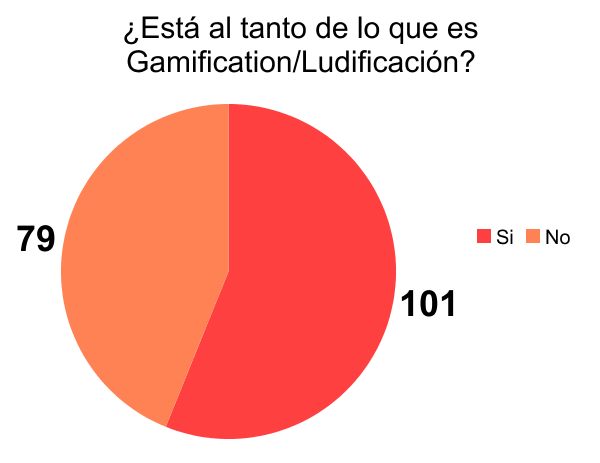
\includegraphics[width=0.5\textwidth]{images/chart3.png}
  \caption[chart3]{¿Está al tanto de lo que es \emph{Gamification}/Ludificación?}
  \label{fig:chart1}
\end{figure}

Le pregunta siguiente, numero $4$, se realizo con el motívo de reforzar el entendimiento de la pregunta
anterior. En esta se obtiene un resultado similar, en donde un $56\%$ contesta positivamente a la
pregunta ""¿Usted acumula puntos de grandes empresas?''. Con esta respuesta se ratifica que existe
conocimiento por parte una la mayoria de los encuestados de la existencia de esta tecnica y que han
interactuado con ella.

\begin{figure}[!htb]
  \centering
  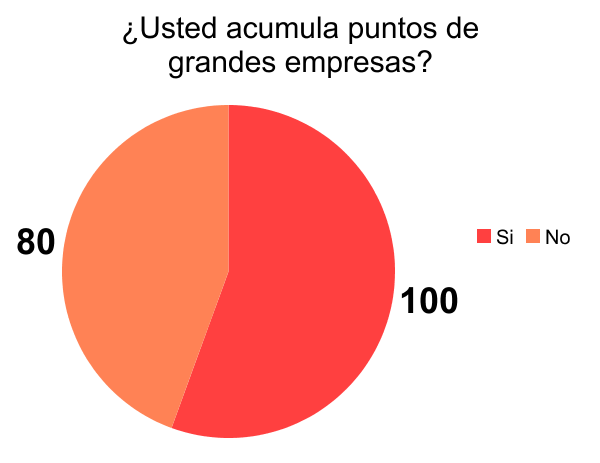
\includegraphics[width=0.5\textwidth]{images/chartPreg4.png}
  \caption[chart4]{¿Usted acumula puntos de grandes empresas?}
  \label{fig:chart2}
\end{figure}

Las preguntas $5$ y $6$ son exclusivas para las personas que si acumulan puntos de diversas formas.Estas
eran las unicas preguntas opcionales y por esto tienen universos diferentes.
En la primera existen $92$ encuestados que contituyen el $100\%$. Esta tiene como objetivo conocer
si los encuestados estan en conocimiento de los beneficios entregados por las empresas a cambio de
 los puntos acumulados. Con $69$ personas contestando positivamente, equivalente a $75\%$, se puede
apreciar que los encuestados tienen un proposito o motivo por lo cual seguir comprando, en este caso
los beneficios entregados.
La siguiente tiene un universo de $101$ personas, del cual un $78\%$ contesto con un ``si'' y el
restante $22\%$ de forma negativa. Con esto se remarca que los encuestados estan en conocimiento
de toda la informacion necesaria para motivarlos a seguir y conquistar su meta, intercambiar sus
puntos por beneficios.

\begin{figure}[!htb]
  \centering
  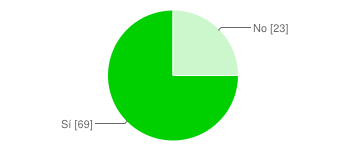
\includegraphics[width=0.5\textwidth]{images/chartPreg5.png}
  \caption[chart5]{¿Está al tanto de los beneficios que dicha empresa le ofrece?}
  \label{fig:chart2}
\end{figure}


\begin{figure}[!htb]
  \centering
  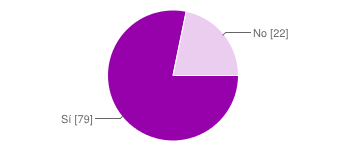
\includegraphics[width=0.5\textwidth]{images/chartPreg6.png}
  \caption[chart6]{¿Ha utilizado éstos beneficios en algún momento?}
  \label{fig:chart2}
\end{figure}

La siguiente pregunta, $7$, tiene como objetivo conocer los beneficios mas atractivos para el ususario.
Esta constaba de una escala de 1 a 5, 1 siendo el menos interesante y 5 el más interesante, en la cual
el beneficio con mas respuestas $5$, o mas interesante para los encuestados, es la obtencion de
descuentos en dinero con un $79\%$. El siguiente beneficio con mas interes es la adquisicion de descuentos
para proximas compras con un $32\%$ de los encuestados. Una informacion importante obtenida es que
una de las herramientas mas utilizadas, obtencion de puntos, es resentida por las personas debido a
que existe un mayor rechazo, $22\%$, que aceptacion, $18\%$, pero la diferencia no es sustantiva para
descartarla como metodo a utilizar. El beneficio mas rechazado, mayor cantidad de $1$, fue la
obtencion de un reconocimiento por tabla de posiciones con un $81\%$.

\begin{figure}[!htb]
  \centering
  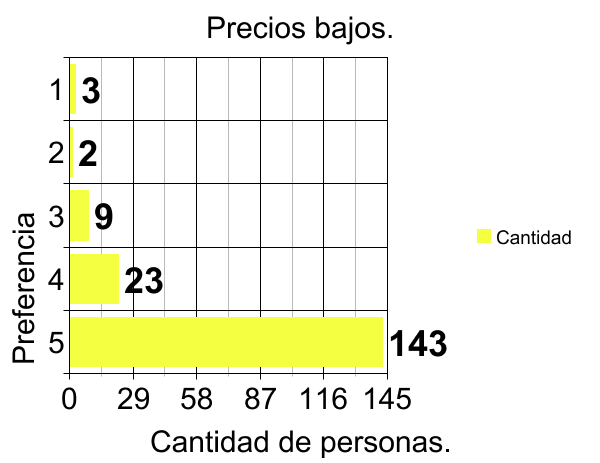
\includegraphics[width=0.5\textwidth]{images/chartPreg7_1.png}
  \caption[chart7-1]{¿Qué beneficios prefiere o preferiría obtener? - Precios bajos.}
  \label{fig:chart2}
\end{figure}

\begin{figure}[!htb]
  \centering
  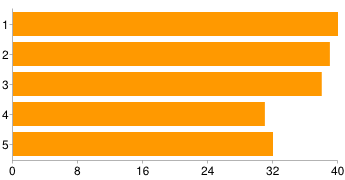
\includegraphics[width=0.5\textwidth]{images/chartPreg7_2.png}
  \caption[chart7-2]{¿Qué beneficios prefiere o preferiría obtener? - Descuentos en próximas compras.}
  \label{fig:chart2}
\end{figure}

\begin{figure}[!htb]
  \centering
  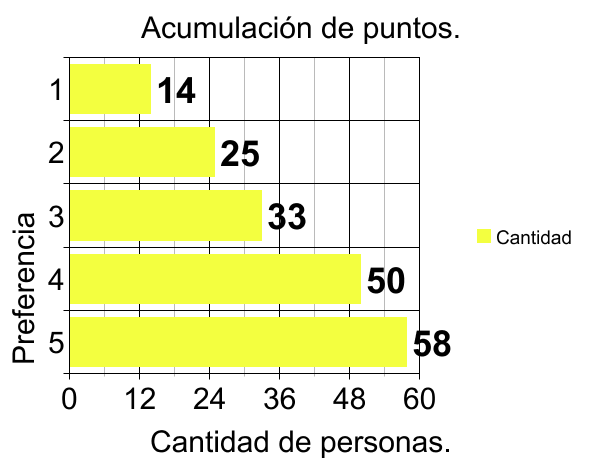
\includegraphics[width=0.5\textwidth]{images/chartPreg7_3.png}
  \caption[chart7-3]{¿Qué beneficios prefiere o preferiría obtener? - Acumulación de puntos.}
  \label{fig:chart2}
\end{figure}

\begin{figure}[!htb]
  \centering
  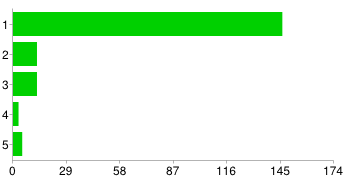
\includegraphics[width=0.5\textwidth]{images/chartPreg7_4.png}
  \caption[chart7-4]{¿Qué beneficios prefiere o preferiría obtener? - Reconocimiento publico según tabla de posiciones.}
  \label{fig:chart2}
\end{figure}

La pregunta $8$ muestra cual es la preferencia a la hora de comprar, presencial u online. La preferencia
mas seleccionada, por $134$ personas, fue la opcion de compra presencial. Esto indica que en Chile
no se acostumbra a comprar via internet y esto representa una oportunidad de negocio debido al
incremento de alfabetizacion digital y con esto el aumento del uso de internet.

\begin{figure}[!htb]
  \centering
  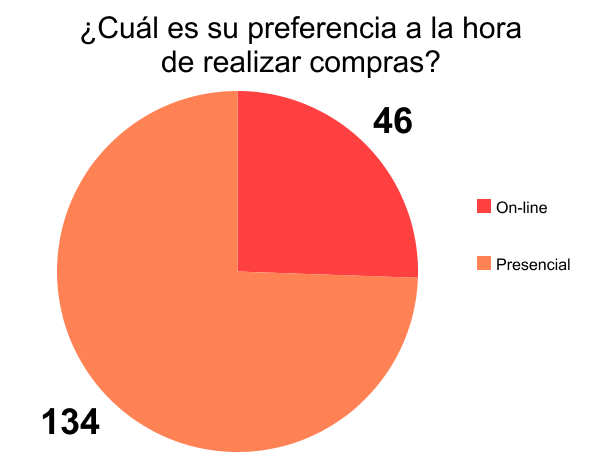
\includegraphics[width=0.5\textwidth]{images/chartPreg8.png}
  \caption[chart8]{¿Cuál es su preferencia a la hora de realizar compras?}
  \label{fig:chart2}
\end{figure}

Una vez respondida la pregunta anterior se le expone al usuario, en la pregunta $9$,  preferiria
utilizar un sitio de ventas online convencional, solo es utilizado para la trasaccion entre cliente
y empresa, o un sitio el cual le ofresca herramientas de \emph{gamification}. Con un $69\%$ seleccionan
una tienda con \emph{gamification} como la alternativa preferida. Con este resultado se apoya la
utilizacion de este concepto con el fin de atraer a nuevos usuarios.

\begin{figure}[!htb]
  \centering
  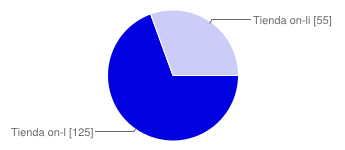
\includegraphics[width=0.5\textwidth]{images/chartPreg9.png}
  \caption[chart9]{¿Prefiere un sitio de ventas on-line con "Gamification" o un sitio convencional?}
  \label{fig:chart2}
\end{figure}

La pregunta $10$ intenta ratificar una de las mayores ideas tras la utilizacion de \emph{gamification},
la motivacion que se crea en el usuario. Se obtuvo que $122$ personas crean esta motivacion
para volver a utilizar o comprar la tienda lo cual es bastante importante al momento de implementar
una solucion gamificada y aun mas cuando se trata de comercio electronico.

\begin{figure}[!htb]
  \centering
  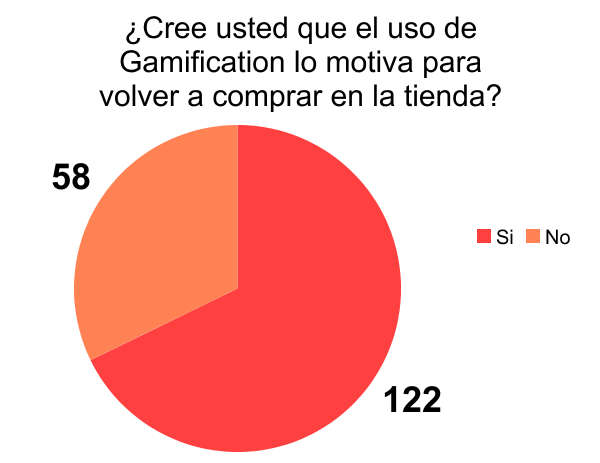
\includegraphics[width=0.5\textwidth]{images/chartPreg10.png}
  \caption[chart10]{¿Cree usted que el uso de \emph{Gamification} lo motiva para volver a comprar en la tienda?}
  \label{fig:chart2}
\end{figure}

Por ultimo se intenta obtener una idea de que contextos podian ser interesante para implementar una
solucion gamificada. La mas votada fue el contexto social con $109$ preferencias, seguida por educación con
$100$ encuetados. Esta pregunta tenia como objetivo dar alguna idea sobre trabajos futuros a realizar.

\begin{figure}[!htb]
  \centering
  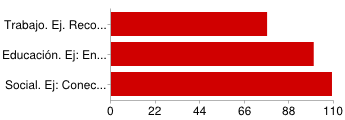
\includegraphics[width=0.5\textwidth]{images/chartPreg11.png}
  \caption[chart11]{¿En que contexto estaría dispuesto al uso de \emph{Gamification}?}
  \label{fig:chart2}
\end{figure}
